\chapter{实验评估}
\section{实验设置}
本次实验的实验环境为Windows 10 64位的系统,CPU为四核Intel Xeon 3.3Ghz CPU,24G内存。代码实现环境为Python3.5配合TensorfFow1.8.0版本。

TensorFlow是谷歌旗下的一款深度学习框架, 是一个使用数据流图进行数值计算的开放源代码软件库,利用TensorFlow框架可以轻松实现深度学习模型而不需要考虑算法的底层实现,并且TensorFlow提供多个优化器可供选择,其灵活的参数设置机制让使用者能够快速调整深度学习模型。因为其方便性与易用性,TensorFlow已经成为了机器学习工作者实现其模型的首选框架,这也是本文采用TensorFlow实现稳中算法的原因。

本文采用的数据集共12780个样例,其中5340个样例为不含空指针的正确代码,7440个样例为含空指针的缺陷代码。由于对于无缺陷代码的检测率四个工具检测准确率都较高,区分度较小,训练数据时限制了正确代码的数量,随机抽取了1000了个样例进行训练。去除掉一些节点数量异常大和数据过于稀疏的样例,总共有7638个样例进行训练,对于训练集数据,各个工具的检测结果分布如表\ref{tt}:

\begin{table}[ht]
	\centering
	\caption{训练集上工具检测结果}
	\label{tt}
	\begin{tabular*}{0.9\textwidth}{@{\extracolsep{\fill}}cccc}
		\toprule
		工具	&正确数量&错误数量&准确率	 \\
		\midrule
		FindBugs&5834&1488&76.68\%\\
		Infer&5102&2761&64.89\%\\
		Jlint&4964&2855&63.49\%\\
		Fortify&3917&3721&51.28\%\\
		\bottomrule
	\end{tabular*}
\end{table}

从上表可以看到即使是准确率最低的工具Fortify也达到了50\%以上的准确率,如果直接将这批训练集放入模型训练的话,因为正负样本数量分布不均的情况,很容易出现模型直接收敛到样本多数值的问题,造成最终的模型训练效果低下。为了解决样本分布不均的问题,本文试验了两种常用的方法,过采样和欠采样的方法。过采样方法随机重复采样数量较少的样本,从而达到正负样本数量均衡的效果,不过重复的采样容易导致过拟合的问题。欠采样的方法随机丢弃一些多数样本的数据,在训练模型时保持正负样本数据数量的一致。
%依然在浮动图环境中
\begin{figure}[h]
	%盒子一
	\parbox[h]{.5\textwidth}{\centering
		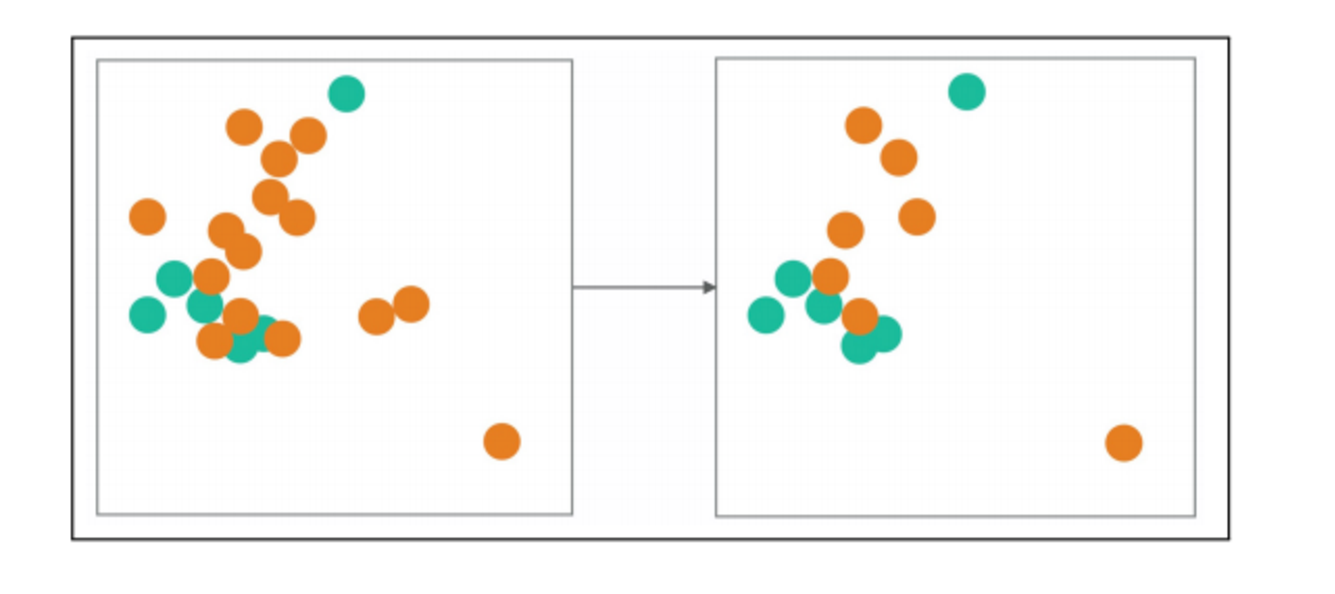
\includegraphics[width=0.45\textwidth]{figures/7.pdf}
		\caption{欠采样方法示例}}
	%盒子二
	\parbox[h]{.5\textwidth}{\centering
		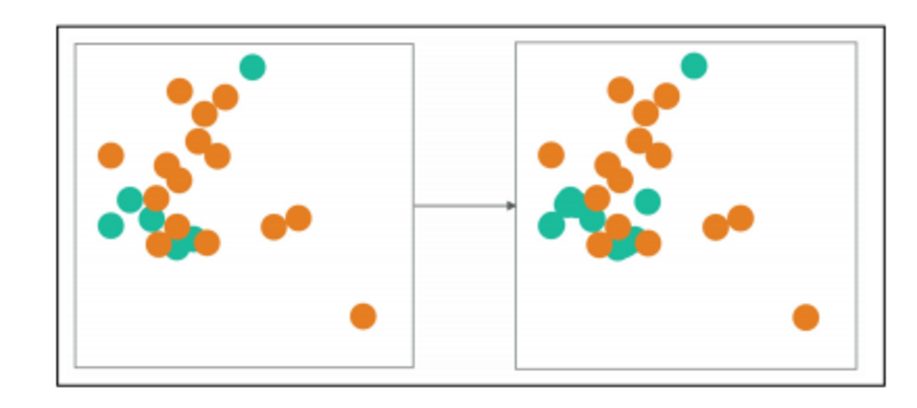
\includegraphics[width=0.45\textwidth]{figures/8.pdf}
		\caption{过采样方法示例}}
\end{figure}

经过对比,本文选择了欠采样的方法。例如针对FindBugs工具,训练时在5834个检测正确的样本中随机挑选出1488个,与1488个缺陷样本一起加入训练,保证了训练数据正负样本的数量均衡。随机欠采样的方法既不会影响数据的统计特征,同时可以使正负样本的边界更为清晰。本文的测试数据采用了不同于训练数据的1000个代码样例,同样的,为了保证样本正负样本数量的均衡,每次测试时,本文从1000个样本中随机抽取正负样本各50个进行测试,测试十次得到测试的平均正确率。

\section{训练设置}
本次模型训练采用了TensorFlow的AdamOptimizer,AdamOptimizer实现了Adam优化算法,比起随机梯度下降的方法,Adam算法收敛速度更加迅速,陷入局部最优解的概率更小。当学习率过大时,容易导致模型发生振荡无法收敛;当学习率过小时,会导致模型收敛速度太慢耗时较长。为了避免上述情况的发生,本文采用了动态学习率的方法。训练学习率初始设置为$10^{4}$,学习率随着训练的迭代步数增加而呈阶梯状下降,每迭代100次变为原来的0.98倍。损失函数采用了交叉熵的算法。对两个概率分布$p$和$q$,通过$q$来表示$q$的交叉熵为:
$$H(p,q) = -\sum_x p(x)\log q(x)$$

通过交叉熵函数可以比较两个概率分布的差异。交叉熵越小,表示两个概率分布差异越小,优化器可以根据交叉熵的值更新模型参数。

针对本文提出的模型,有两个参数可能影响模型的结果:图压缩后特征向量的维度大小$d$以及压缩算法的迭代次数$T$。接下来将分别探讨两者的影响。


对于特征向量$d$,可以看出,当$d$的维度增加,网络中的参数$W_1, W_2, W_3, W_4$的维度都会相应的增加,相当于网络的每一层的神经元都会增加,网络变得更加复杂,能够拟合的函数也就越复杂,于此同时模型的训练难度和时间消耗也会增加。网络如果过于复杂也有可能导致模型过拟合的问题。

对于循环次数$T$,相类似的,随着循环次数的增加,网络的层数逐渐增加,网络更加复杂,拟合的函数越复杂,同时也可能会发生训练时间过长和过拟合的问题。

为了找到最佳的特征向量维度$d$以及迭代次数$T$,本文在迭代次数1到4下特征维度8到512维之间进行了实验。实验采用了相同的训练数据,当模型收敛后对相同的测试集进行测试,得到四个分类器的准确率均值,结果如图\ref{mid}。本文数据采用了图中最佳的组合:循环次数为3,特征向量维度为32维。
\begin{figure}[htbp]
	\begin{center}
		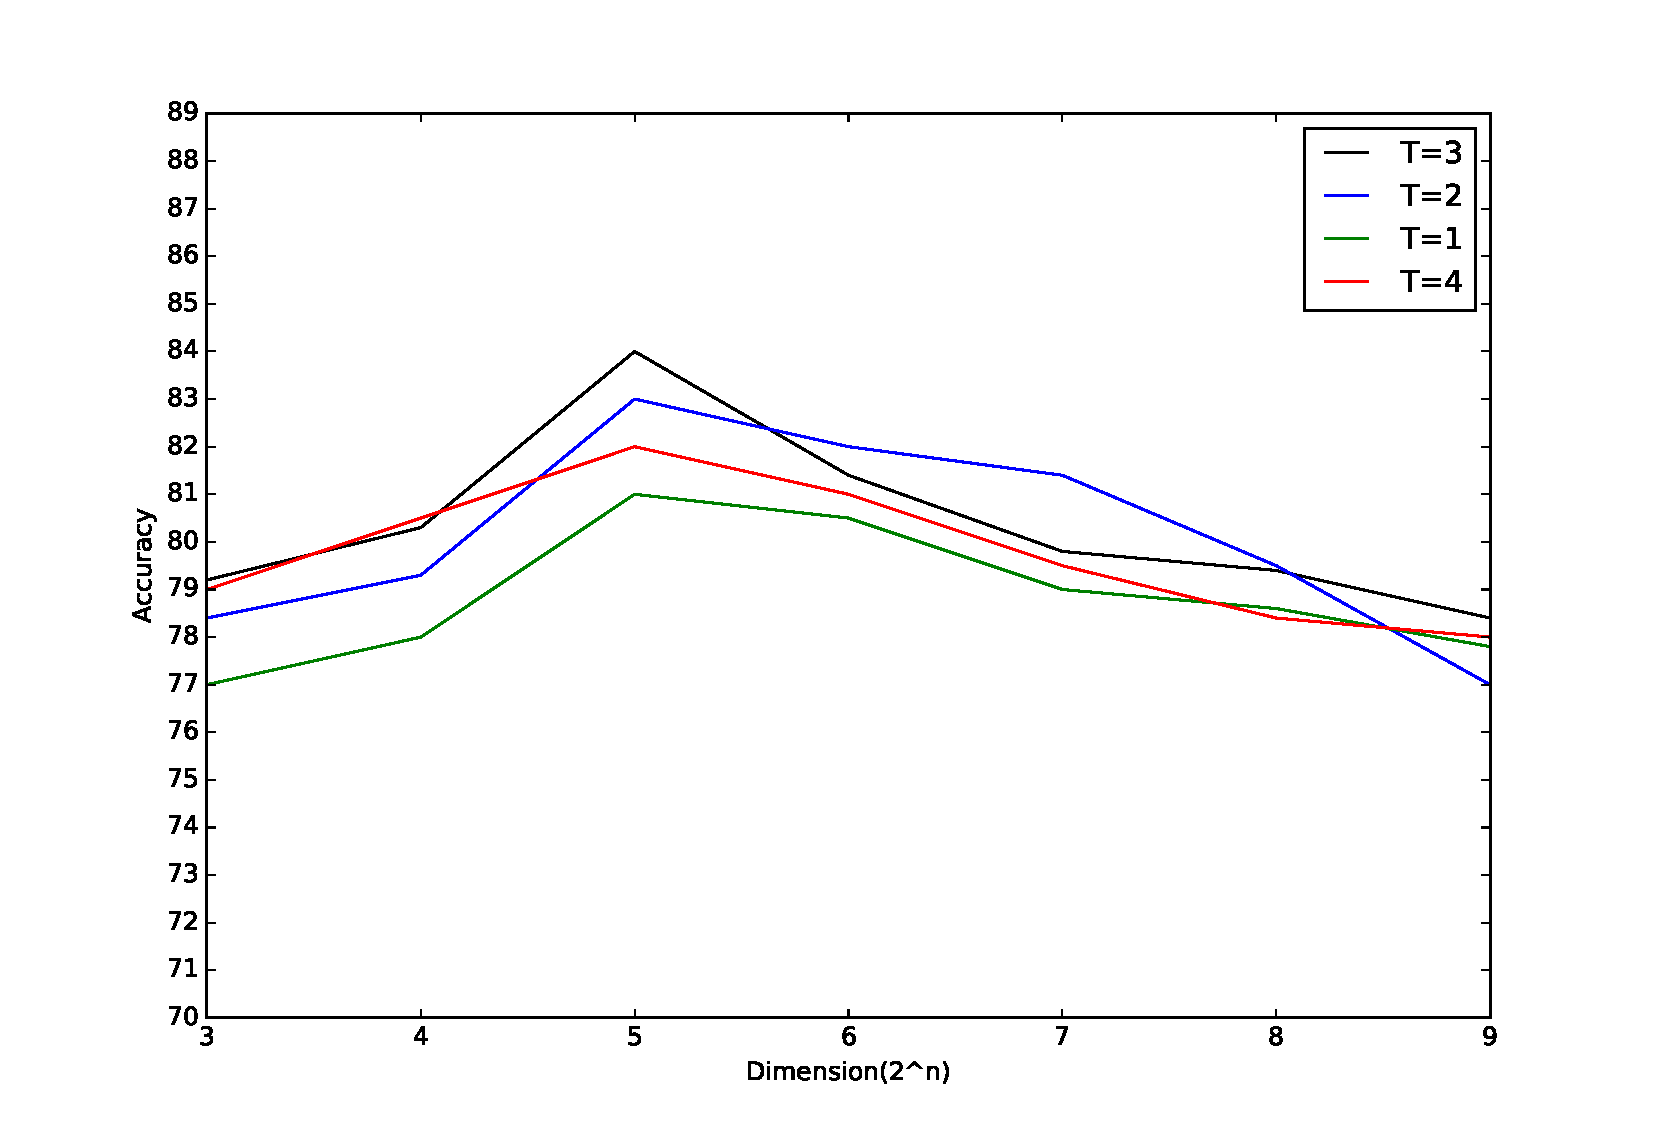
\includegraphics[width=0.95\textwidth]{figures//9.pdf}
		\caption{不同组合的准确率}
		\label{mid}
	\end{center}
\end{figure}
\section{实验结果}
在上文定义好的训练集上进行训练,每一个工具都得到了一个二分类器,分类器在测试集上的准确率达到了80\%以上。为了让实验结果更加清晰,本文对实验结果进行可视化。首先运用训练好的图压缩模型对测试代码控制流图进行压缩得到图特征向量,然后运用t-SNE算法将特征向量压缩为一个二维向量,根据各个工具对该代码检测结果的正确与否给二维向量不同的颜色,得到了图\ref{f1}的结果:

\begin{figure}[h]
\label{f1}
	%盒子一
	\parbox[h]{.5\textwidth}{\centering
		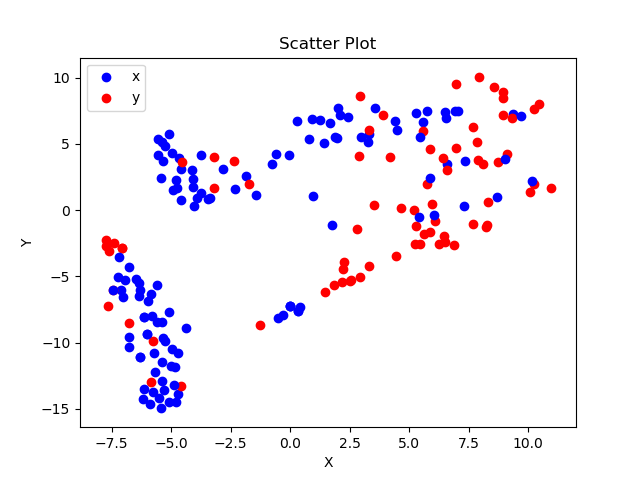
\includegraphics[width=0.45\textwidth]{figures/11.png}
		\caption{FindBugs}}
	%盒子二
	\parbox[h]{.5\textwidth}{\centering
		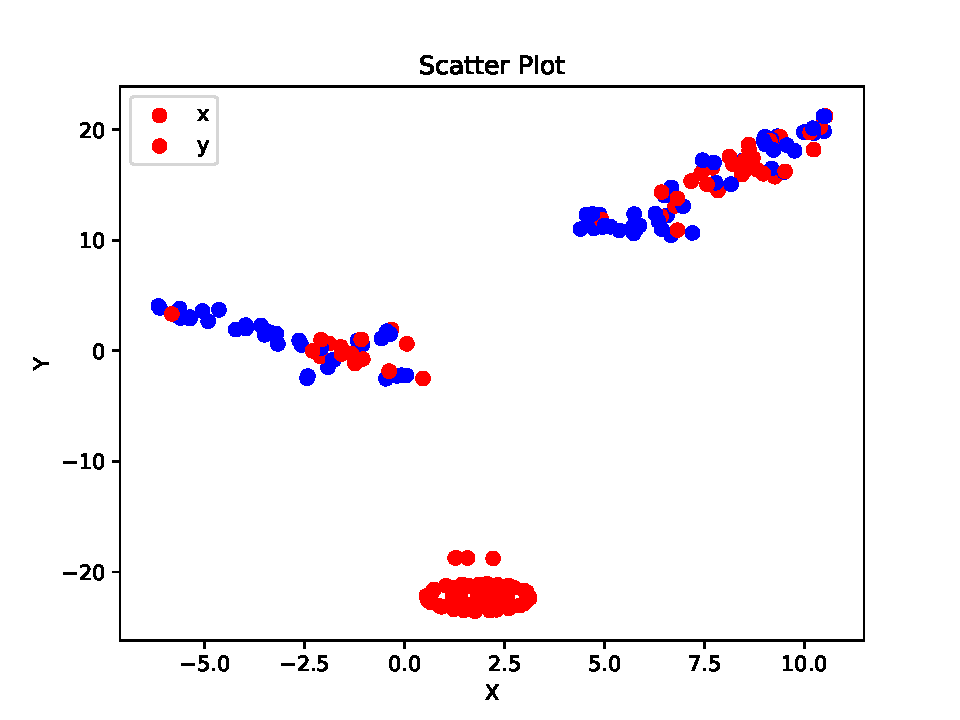
\includegraphics[width=0.45\textwidth]{figures/12.pdf}
		\caption{Infer}}
	\parbox[h]{.5\textwidth}{\centering
		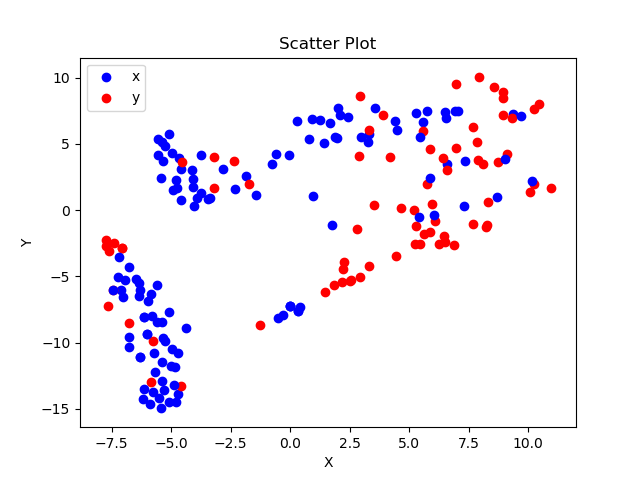
\includegraphics[width=0.45\textwidth]{figures/11.png}
		\caption{Jlint}}
	%盒子二
	\parbox[h]{.5\textwidth}{\centering
		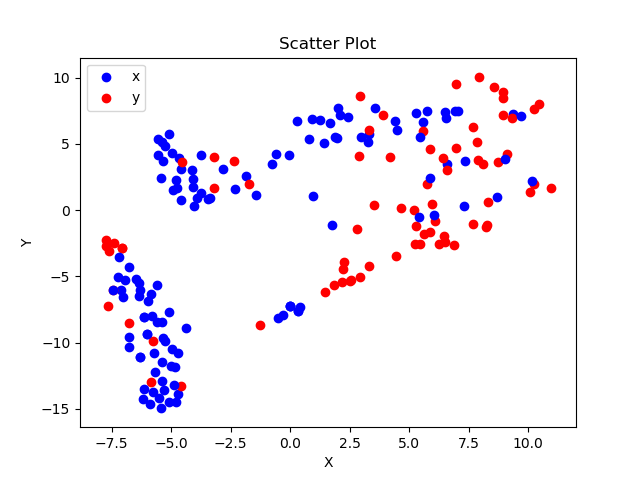
\includegraphics[width=0.45\textwidth]{figures/11.png}
		\caption{Fortify}}
\end{figure}

可以看出FindBugs的点分布比较稀疏,说明了FindBugs的检测规则比较丰富,能够检测的空指针缺陷类型较多;而其他三种工具的点分布呈聚集状,说明其检测所需的特征比较单一,检测的空指针缺陷类型较少。本文中FindBugs的高准确率正好映证了这一点。

四个分类器的ROC曲线如图\ref{roc}:
\begin{figure}[ht]
\label{roc}
	%盒子一
	\parbox[h]{.5\textwidth}{\centering
		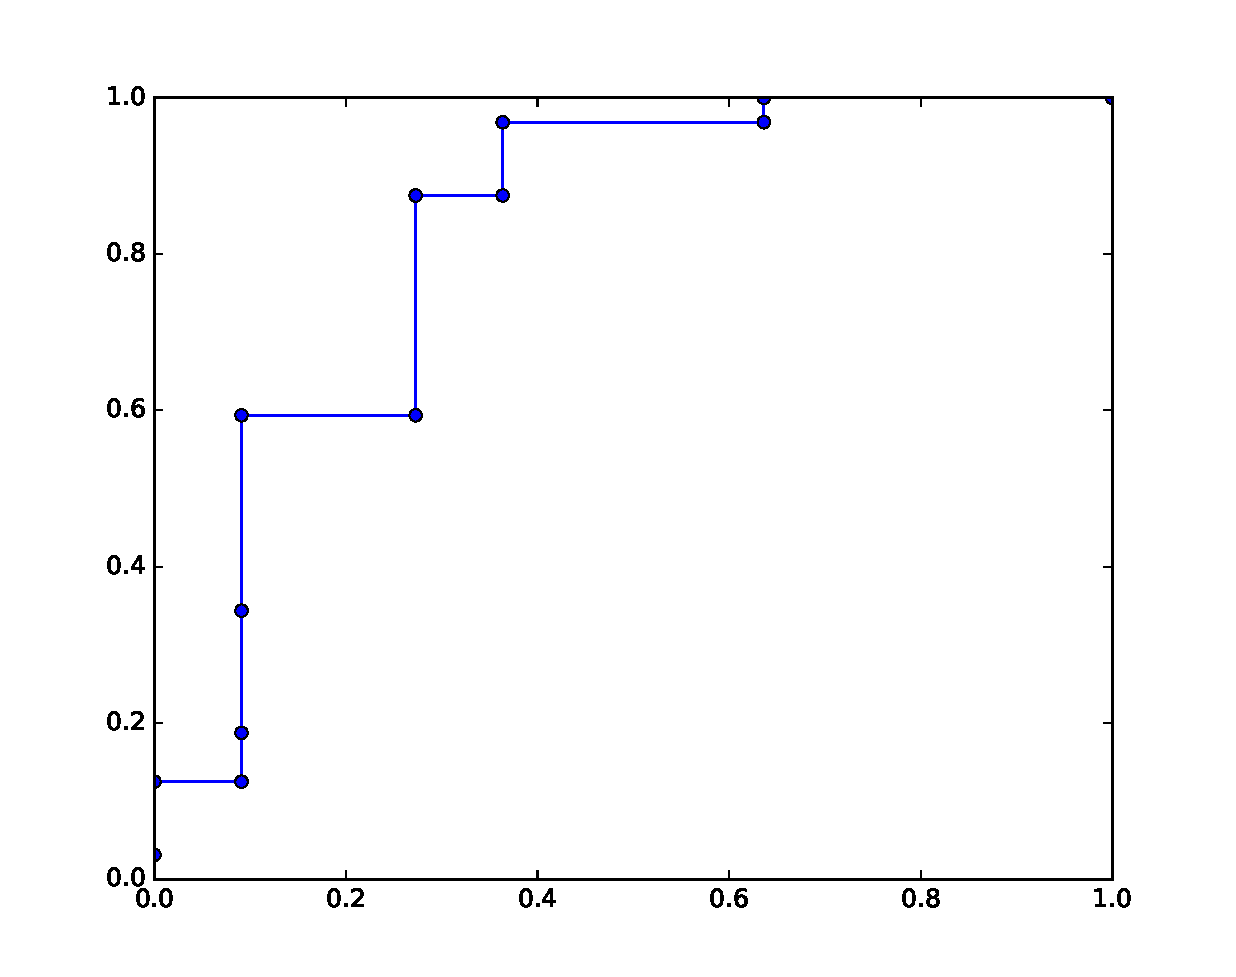
\includegraphics[width=0.45\textwidth]{figures/13.pdf}
		\caption{FindBugs}}
	%盒子二
	\parbox[h]{.5\textwidth}{\centering
		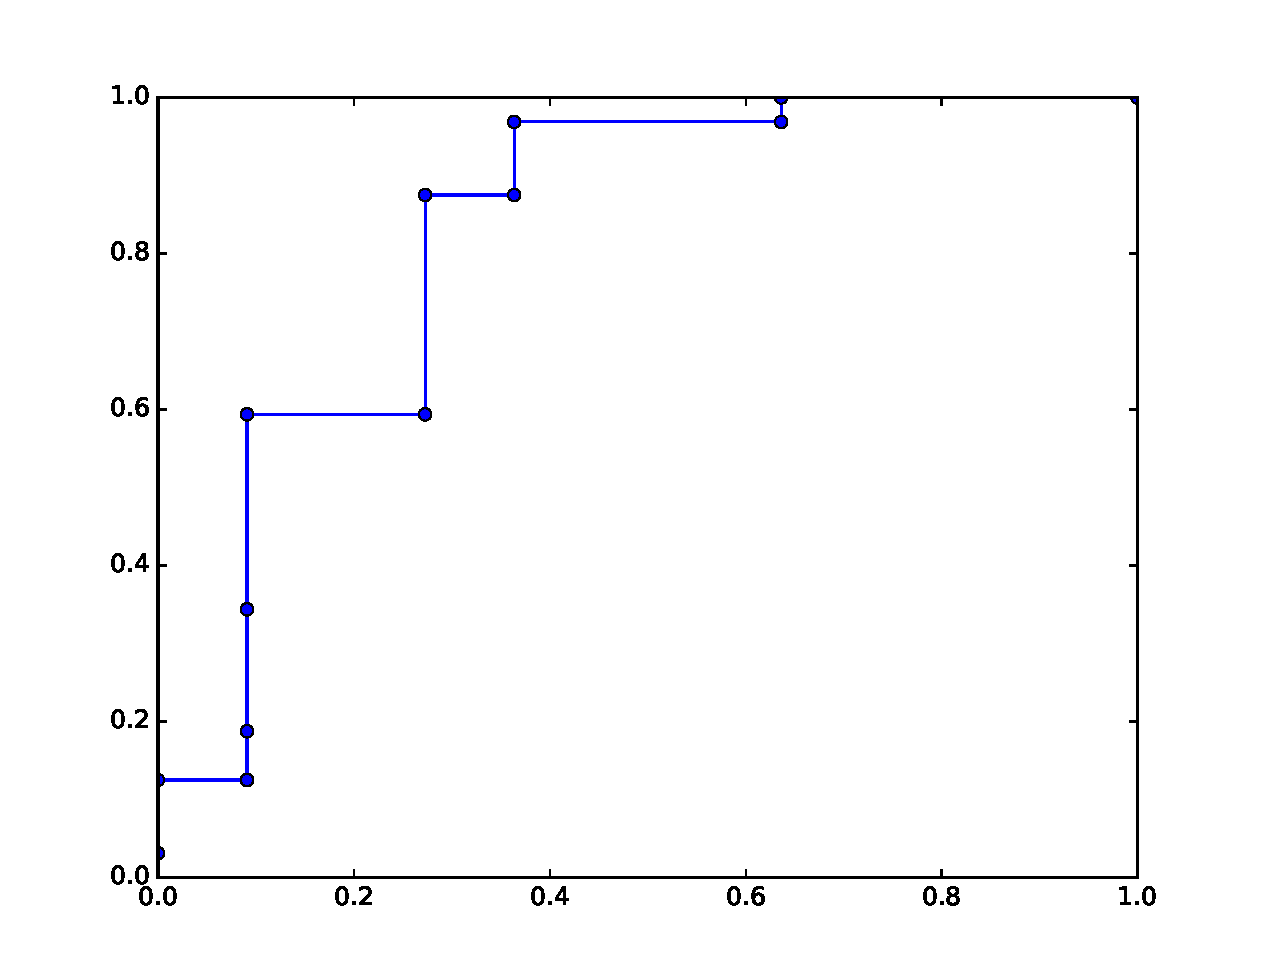
\includegraphics[width=0.45\textwidth]{figures/14.pdf}
		\caption{Infer}}
	\parbox[h]{.5\textwidth}{\centering
		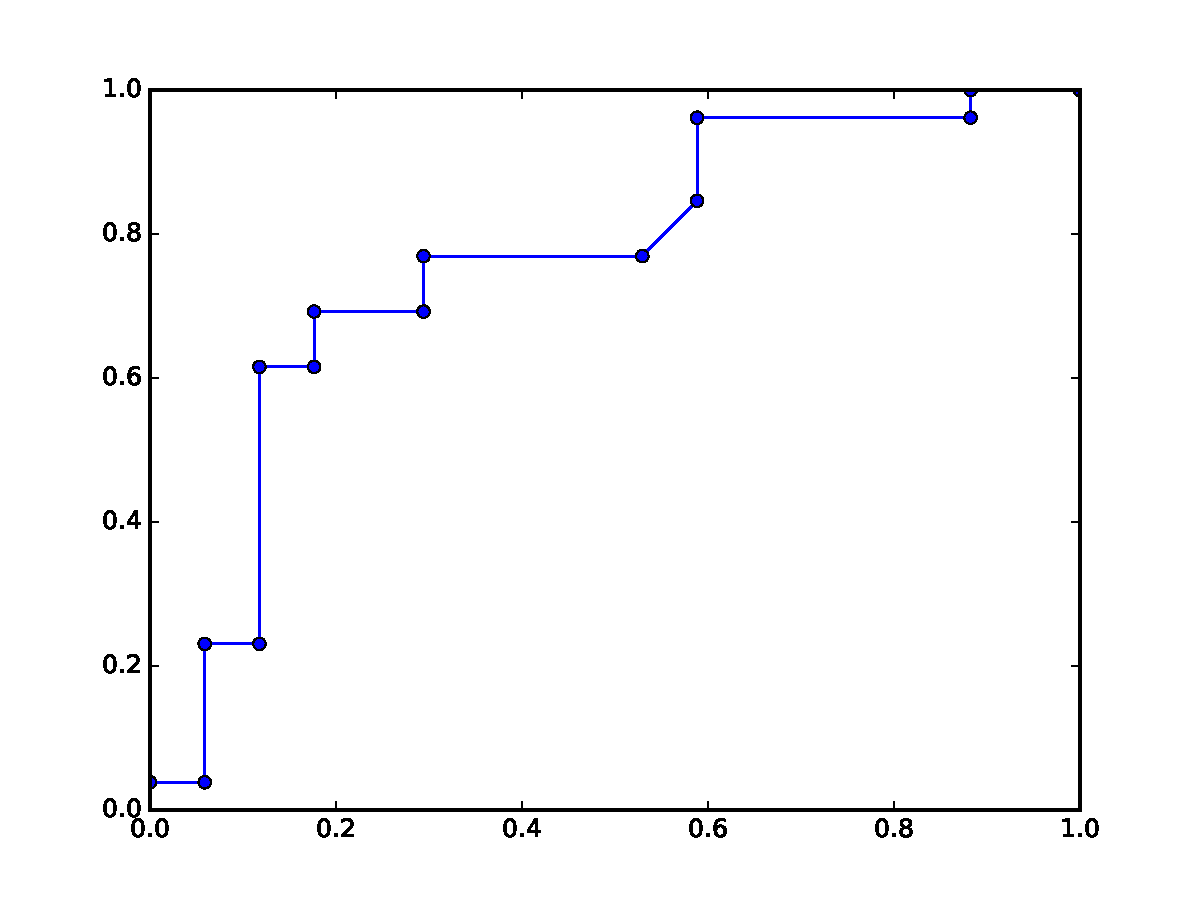
\includegraphics[width=0.45\textwidth]{figures/15.pdf}
		\caption{Jlint}}
	%盒子二
	\parbox[h]{.5\textwidth}{\centering
		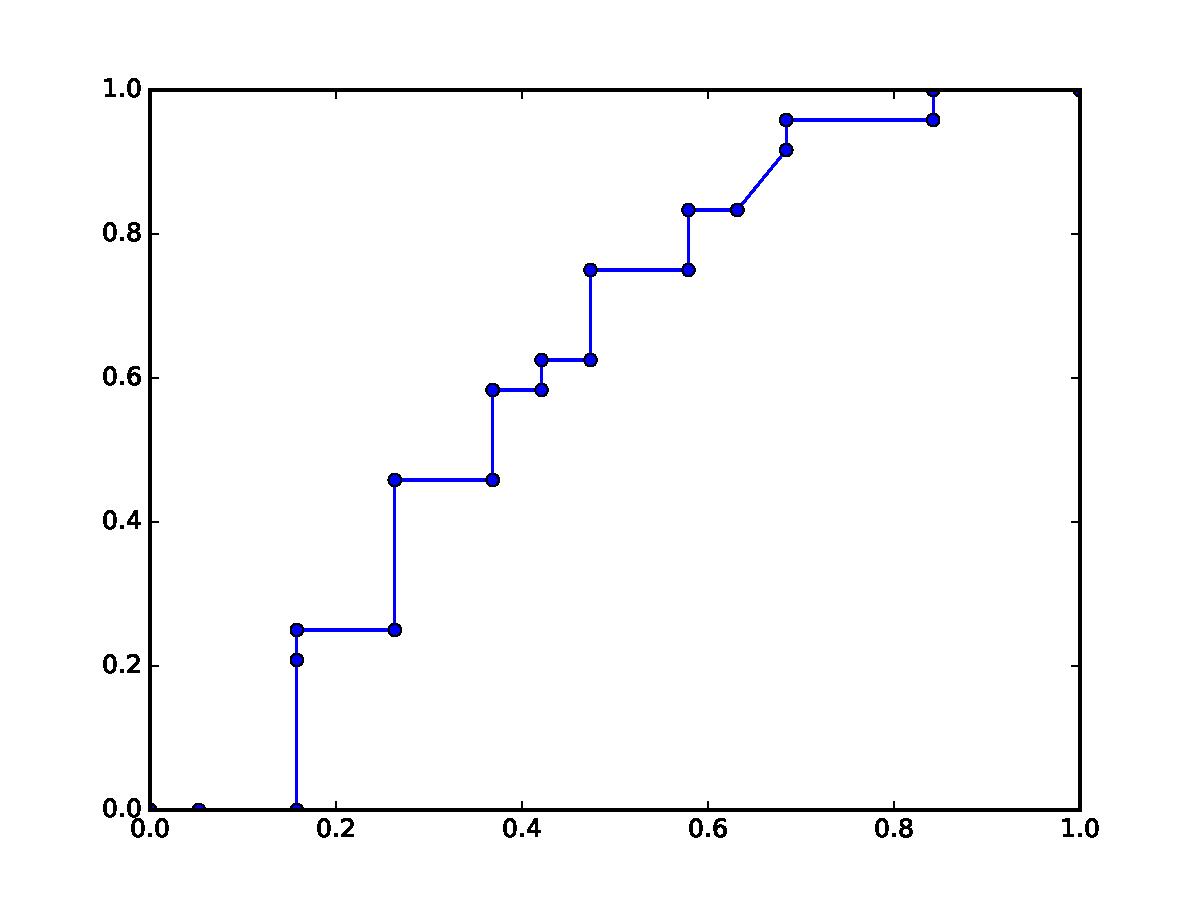
\includegraphics[width=0.45\textwidth]{figures/16.pdf}
		\caption{Fortify}}
\end{figure}


得到四个分类器后,可以综合分类器的结果和四个工具的检测结果进行空指针判定。为了增加工具检测含空指针和不含空指针数据之间的差异,本文对标签进行了预处理,当工具检测含空指针时,置为1;工具检测不含空指针时,置为0。这样得到四个工具的检测结果向量$R={r_1, r_2, r_3, r_4}$,模型得出的四个工具的置信度矩阵$W={w_1, w_2, w_3, w_4}$,这样测试样例是否含有空指针的置信度为$P = W^T*R = \sum_{i=1}^4 w_i*r_i$。这样可以充分利用工具和分类器的结果,并且具有一定的容错性,当一个分类器出现预测错误时,其他三个分类器的结果可以弱化此分类器的错误,从而最小化单个分类器的错误对整个判定模型的影响。为了实现空指针检测结果的最终判定,可以设定一个阈值$p$, 当$P>=p$时判定该代码存在空指针缺陷。

当模型分类完全没有误差时,阈值$p$应该接近于0。然而在现实中模型无法做到没有偏差,因此$p$的值并不能单纯取0,为了得到$p$最佳的取值,本文选取了从-0.3到0.4,每隔0.05取一个阈值进行实验。实验从测试集中随机选取了100个样例,对这100个样例进行空指针检测以及模型检验,计算空指针检测准确率后得到表\ref{res}的结果:
\begin{figure}[ht]
	\begin{center}
		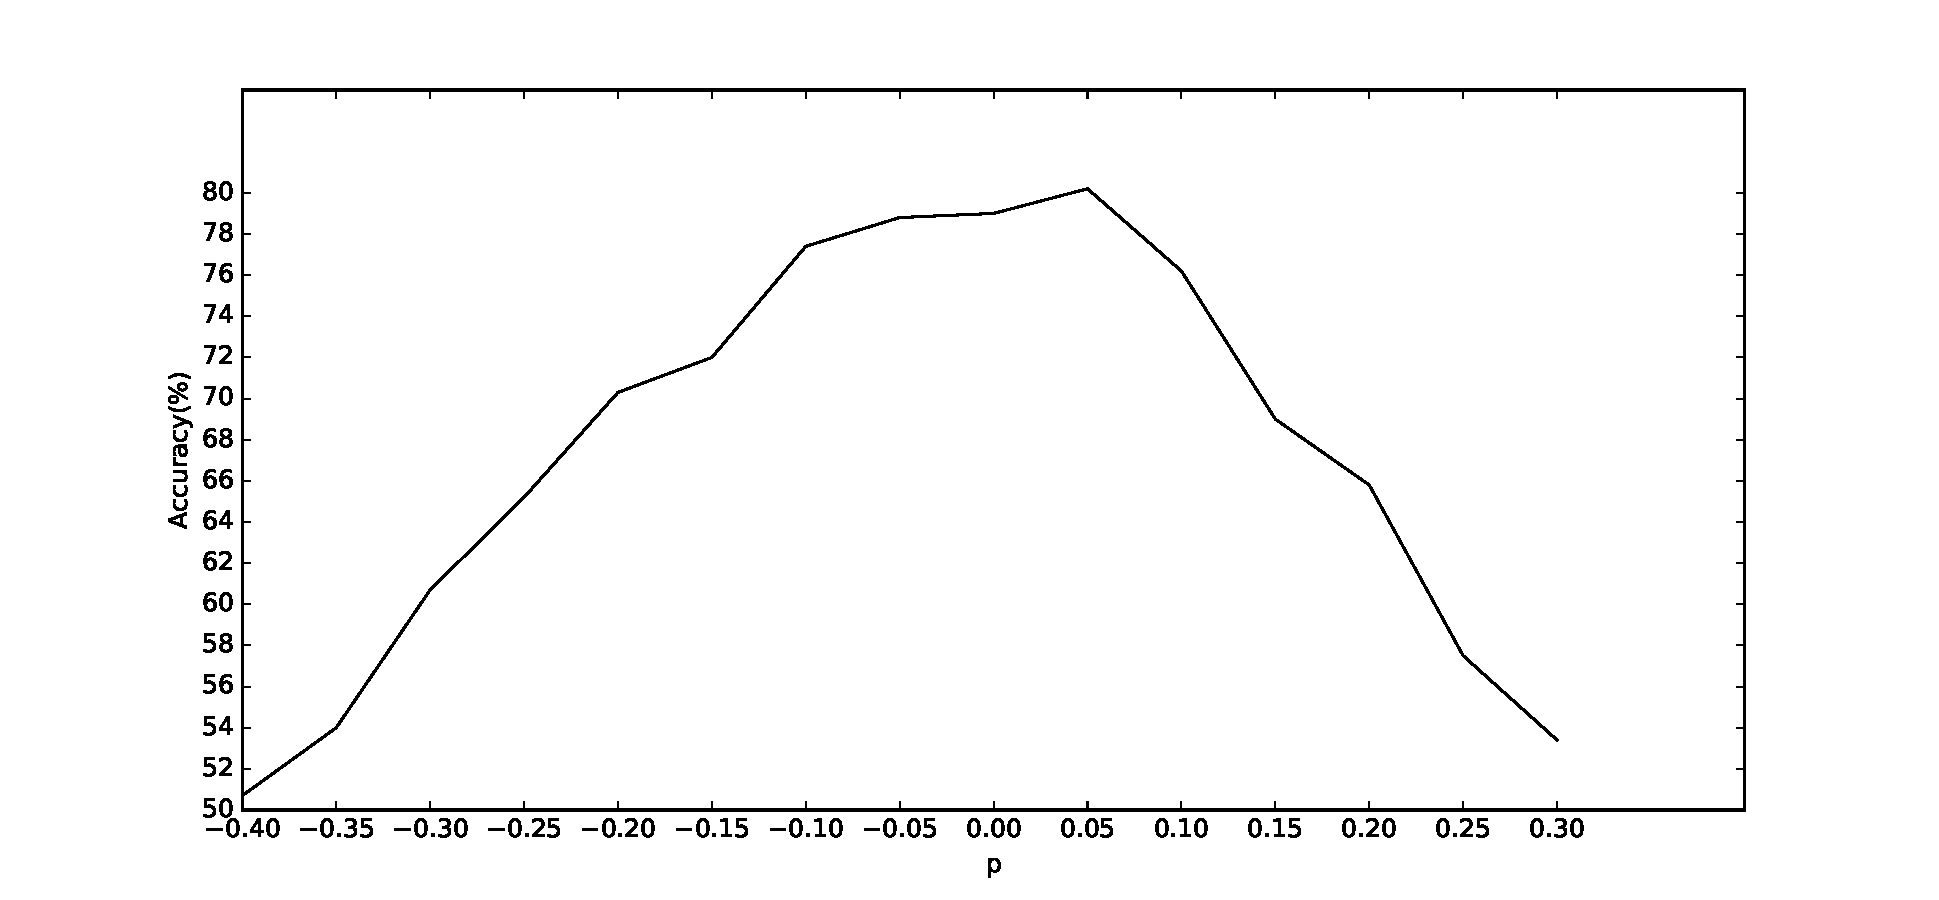
\includegraphics[width=0.95\textwidth]{figures//10.pdf}
		\caption{不同阈值下的空指针检测准确率}
		\label{res}
	\end{center}
\end{figure}

可以看到当阈值为0.05时能够取得最大的检测准确率81.34\%。这说明了模型的预测结果较为保守,而阈值的选取正好中和了其中的偏差,从而使模型的总体准确率超过了所有的静态检测工具。